\section{Parser}

Każdy z dokumentów HTML'a musi zawierać znaczniki typowe dla tego formatu, których nie znajdziemy w dokumentach \LaTeX. Są to: \textbf{\textit{html}},
\textbf{\textit{head}} oraz \textbf{\textit{body}}. Jako odpowienik sekcji \textbf{\textit{head}} przyjęliśmy sekcję preambuly w której 
znajdują się między innymi takie polecenia jak \textit{usepackage}. Natomiast jak odpowiednik sekcji \textbf{\textit{body}} odpowiada fragment kodu 
\LaTeX \space objęty poleceniami \textit{begin\{document\}} oraz \textit{end\{document\}}.

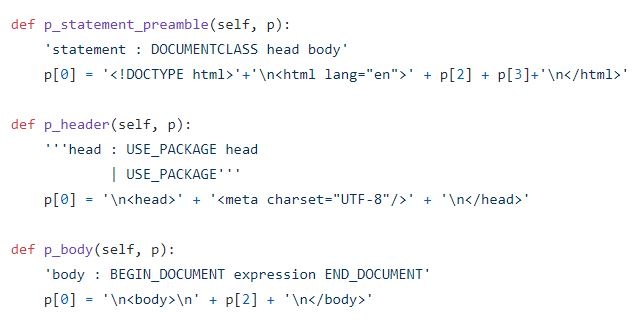
\includegraphics{preamble.JPG}

\subsection{Obsługa tekstu}

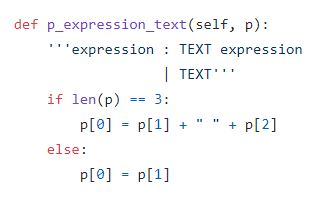
\includegraphics{expression_text.JPG}

\subsection{Formatowanie tekstu}

Nasz translator umożliwia pogrubienie, kursywa, podkreślenie, wyśrodkowanie tekstu oraz utworzenie paragrafu. Możliwe jest mieszanie
stylów formatowania, np. pogrubienie z podkreśleniem. Według nowych zaleceń, do pogrubienia tekstu w HTMLu powinno się stosować znacznik
"strong", a do kursywy "em".

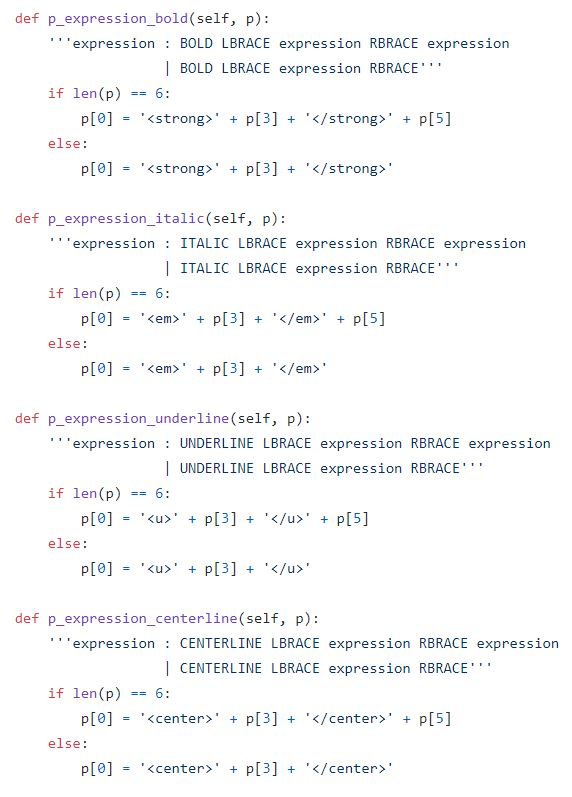
\includegraphics{bold_italic_underline_centerline.JPG}

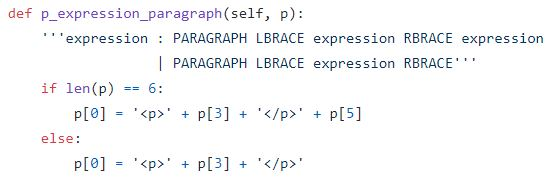
\includegraphics{paragraph.JPG}


Kolejną funkcjonalnością jest możliwość obsługi rozdziałów, sekcji i podsekcji parsując znaczniki chapter, section, subsection, 
subsubsection.


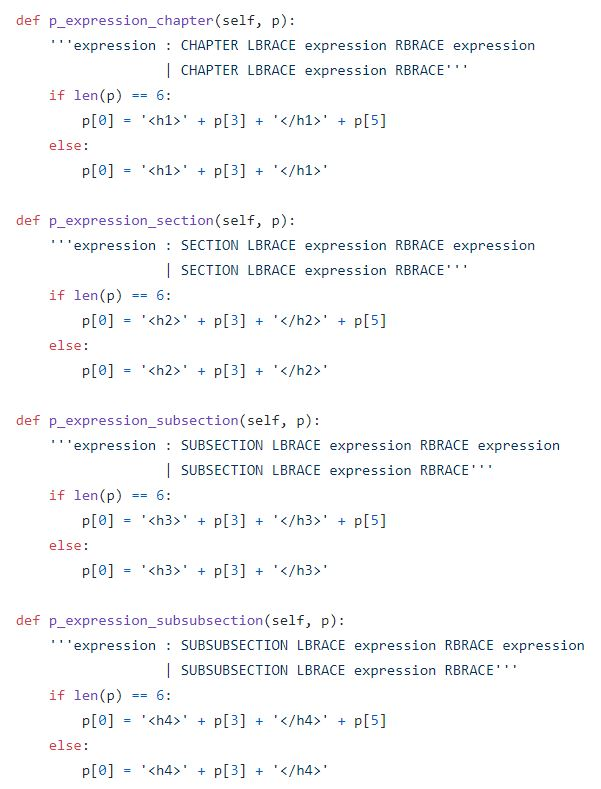
\includegraphics{chapter_section.JPG}


Przejście do nowej linii (hard break) jest obsłużony poleceniem newline.

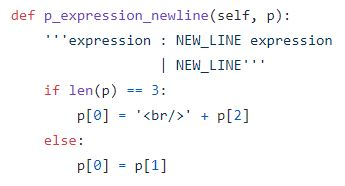
\includegraphics{newline.JPG}


Translator parsuje również znacznik title odpowiadjący z utworzenie tytułu.

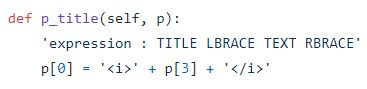
\includegraphics{title.JPG}

\subsection{Tabela}

\subsubsection{Z obramowaniem}

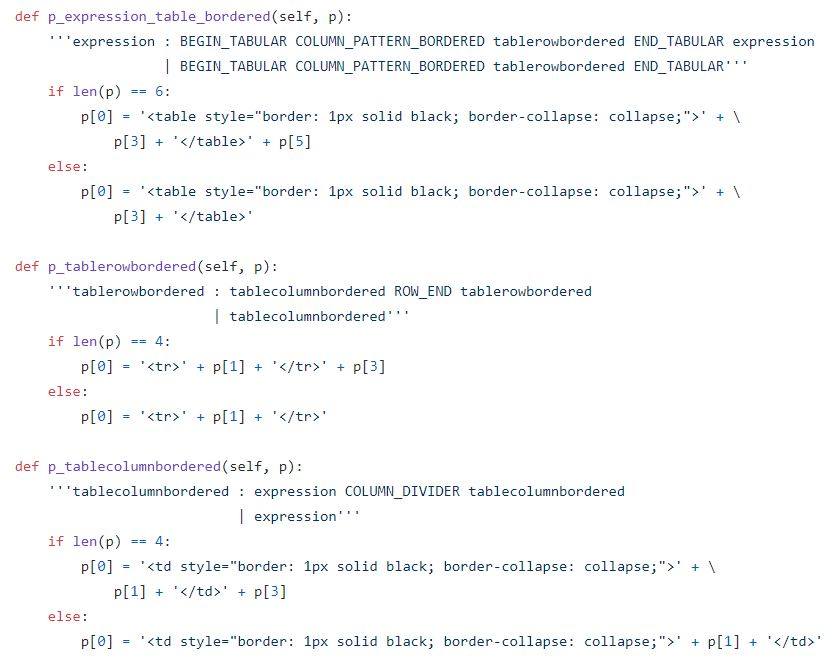
\includegraphics{table_bordered.JPG}

\subsubsection{Bez obramowania}

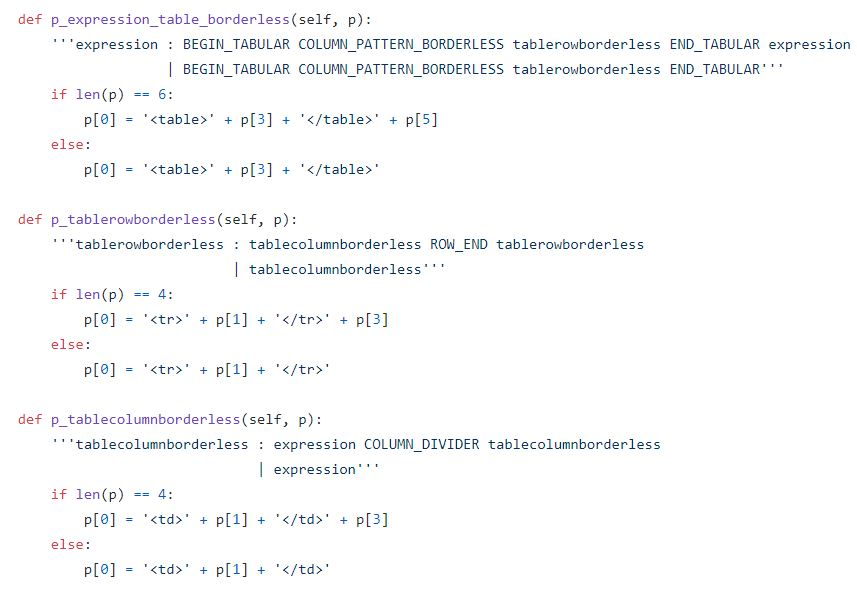
\includegraphics{table_borderless.JPG}


\subsection{Wyliczenie}

Konstrukcja parsera wyliczeń umożliwia wykonywanie zagnieżdżeń.

\subsubsection{Uporządkowane}

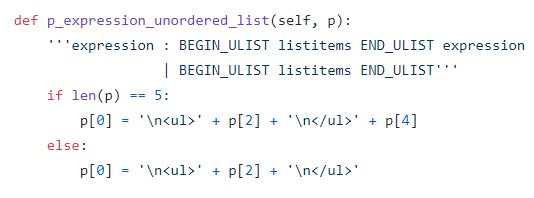
\includegraphics{unordered_list.JPG}

\subsubsection{Nieuporządkowane}

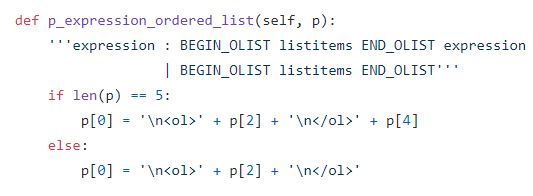
\includegraphics{ordered_list.JPG}

\subsection{Grafika}

Umieszcznie grafiki jest możliwe dzięki znacznikowi "includegraphics" w LaTeX, który jest parsowany na znacznik "img" w HTML, gdzie 
atrybut :src" stanowi ścieżka do pliku umieszczona w nawiasach wąsatych w dokumencie LaTeX.

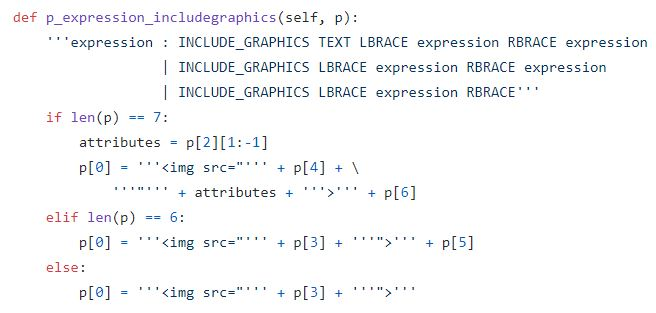
\includegraphics{includegraphics.JPG}

\subsection{Hiperłącze}

Zamieszczenie hiperłącza w formacie LaTeX jest możliwe dzięki znacznikowi "url", zawierającego w nawiasach wąsatych adres do strony.
Parsowanny jest on na HTMLowy znacznik "a" z atrybutem "href" zawierającego adres.

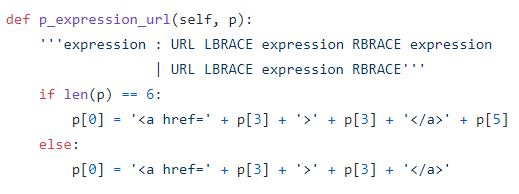
\includegraphics{url.JPG}